\documentclass[tikz,border=10pt]{standalone}
\usepackage{amsmath}
\usepackage{amsfonts}
\usepackage{amssymb}
\usetikzlibrary{shapes.geometric, arrows.meta, positioning, fit, backgrounds, calc}

\begin{document}

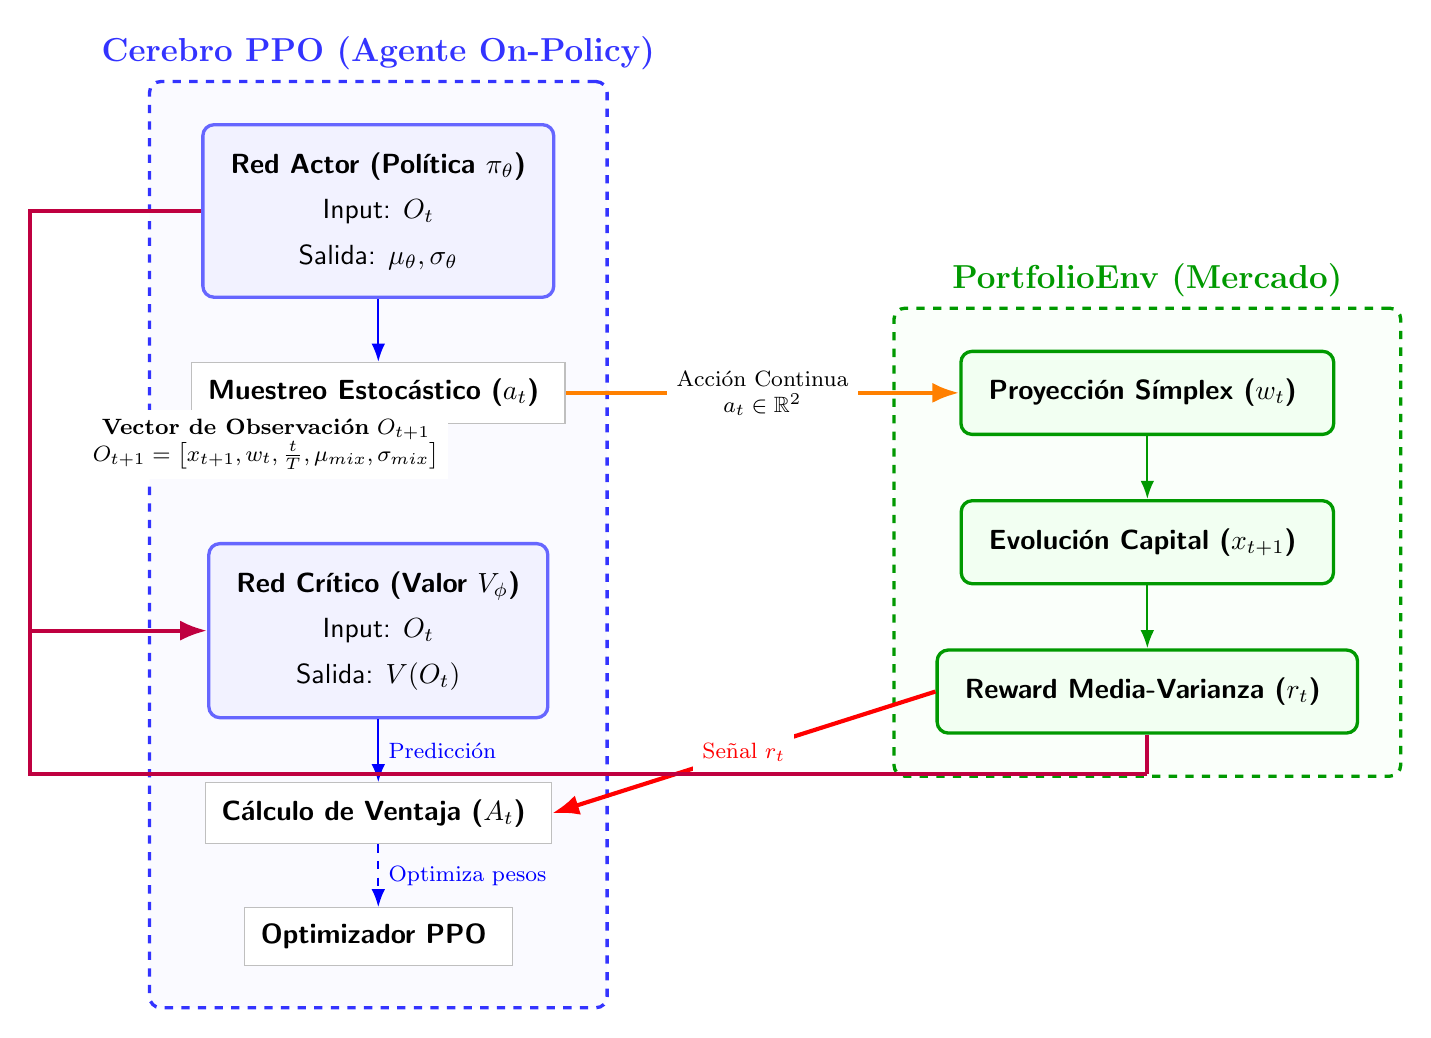
\begin{tikzpicture}[
    >=Latex,
    node distance=1.5cm and 2cm,
    font=\sffamily,
    % Estilos de cajas
    agentbox/.style={rectangle, rounded corners, draw=blue!60, fill=blue!5, very thick, align=center, inner sep=10pt},
    envbox/.style={rectangle, rounded corners, draw=green!60!black, fill=green!5, very thick, align=center, inner sep=10pt},
    mathbox/.style={rectangle, draw=gray!50, fill=white, align=center, inner sep=6pt},
    arrowlabel/.style={fill=white, text=black, font=\footnotesize, align=center}
]

% -------------------------
% AGENTE PPO (Izquierda)
% -------------------------
\node[agentbox] (actor) {
    \textbf{Red Actor (Política $\pi_\theta$)}\\[1ex]
    Input: $O_t$\\[1ex]
    Salida: $\mu_\theta, \sigma_\theta$
};

\node[mathbox, below=0.8cm of actor] (muestreo) {
    \textbf{Muestreo Estocástico ($a_t$)}
};

\node[agentbox, below=1.5cm of muestreo] (critic) {
    \textbf{Red Crítico (Valor $V_\phi$)}\\[1ex]
    Input: $O_t$\\[1ex]
    Salida: $V(O_t)$
};

\node[mathbox, below=0.8cm of critic] (ventaja) {
    \textbf{Cálculo de Ventaja ($A_t$)}
};

\node[mathbox, below=0.8cm of ventaja] (loss) {
    \textbf{Optimizador PPO}
};

% Contenedor del Agente
\begin{scope}[on background layer]
    \node[rectangle, rounded corners, draw=blue!80, fill=blue!2, dashed, very thick, fit=(actor) (muestreo) (critic) (ventaja) (loss), inner sep=15pt, label={[font=\large\bfseries, text=blue!80]above:Cerebro PPO (Agente On-Policy)}] (agent_bg) {};
\end{scope}

% Conexiones internas Agente
\draw[->, thick, blue] (actor) -- (muestreo);
\draw[->, thick, blue] (critic) -- (ventaja) node[midway, right, font=\footnotesize] {Predicción};
\draw[->, thick, blue, dashed] (ventaja) -- (loss) node[midway, right, font=\footnotesize] {Optimiza pesos};

% -------------------------
% ENTORNO (Derecha)
% -------------------------
\node[envbox, right=5cm of muestreo] (proyeccion) {
    \textbf{Proyección Símplex ($w_t$)}
};

\node[envbox, below=0.8cm of proyeccion] (dinamica) {
    \textbf{Evolución Capital ($x_{t+1}$)}
};

\node[envbox, below=0.8cm of dinamica] (recompensa) {
    \textbf{Reward Media-Varianza ($r_t$)}
};

% Contenedor del Entorno
\begin{scope}[on background layer]
    \node[rectangle, rounded corners, draw=green!60!black, fill=green!2, dashed, very thick, fit=(proyeccion) (dinamica) (recompensa), inner sep=15pt, label={[font=\large\bfseries, text=green!60!black]above:PortfolioEnv (Mercado)}] (env_bg) {};
\end{scope}

% Conexiones internas Entorno
\draw[->, thick, green!60!black] (proyeccion) -- (dinamica);
\draw[->, thick, green!60!black] (dinamica) -- (recompensa);

% -------------------------
% INTERACCIONES (Ciclo RL)
% -------------------------
% Acción: Muestreo -> Proyección
\draw[->, line width=1.5pt, orange] (muestreo) -- (proyeccion) node[midway, arrowlabel] {Acción Continua\\$a_t \in \mathbb{R}^2$};

% Reward: Entorno -> Ventaja
\draw[->, line width=1.5pt, red] (recompensa.west) -- (ventaja.east) node[midway, fill=white, font=\footnotesize, align=center] {Señal $r_t$};

% Observación: Entorno -> Actor y Crítico
% Definir punto de salida de observación
\coordinate (obs_out) at ($(recompensa.south) + (0, -0.5)$);
\draw[line width=1.5pt, purple] (recompensa.south) -- (obs_out);
\draw[line width=1.5pt, purple] (obs_out) -| ($(agent_bg.west) + (-1.5, 0)$) |- (actor.west) 
    node[pos=0.15, arrowlabel, xshift=3cm] {\textbf{Vector de Observación} $O_{t+1}$\\$O_{t+1} = \left[x_{t+1}, w_t, \frac{t}{T}, \mu_{mix}, \sigma_{mix}\right]$};

% Derivación de la observación al crítico
\draw[->, line width=1.5pt, purple] ($(agent_bg.west) + (-1.5, 0)$) |- (critic.west);

\end{tikzpicture}
\end{document}
